%ullright document template
%default a4 one-sided article page setup
\documentclass[article, a4paper, oneside, 11pt]{memoir}

%the following three commands are necessary when using pdflatex
%(set input/output encoding)
\usepackage[utf8]{inputenc}
\usepackage[T1]{fontenc}
\usepackage{helvet}
%use sans serife font for body 
\renewcommand*\familydefault{\sfdefault}

%but with more tech-doc like margins
\setlrmarginsandblock{2.8cm}{2.8cm}{*}
\checkandfixthelayout

%for the german language
\usepackage[ngerman]{babel}

%including pictures
\usepackage{graphicx}
\graphicspath{{./figures/}}

%wrapping text around figures
\usepackage{wrapfig}

%provides symbols for shift, enter, etc.
\usepackage{keystroke}

%url handling
\usepackage{url}

%elaborate references
\usepackage[ngerman]{varioref}

%we do not use xelatex anymore
%allows convenient font/color specification
%\usepackage{xcolor}
%\usepackage{fontspec}
%'classic' tex mappings, e.g. -- => en-dash
%\defaultfontfeatures{Mapping=tex-text}
%\setromanfont{Gentium Basic}
%\definecolor{DocBlue}{rgb}{0.1, 0.42, 0.59}
%\setsansfont[Color = DocBlue]{Ubuntu}

\chapterstyle{veelo}
\headstyles{komalike}
\pagestyle{empty}

%header and footer images on every page
\usepackage{wallpaper}
\ULCornerWallPaper{1.0}{header}
\LLCornerWallPaper{1.0}{footer}

%Precise figure placement
% \usepackage{float}

%padding for fbox borders
%\setlength\fboxsep{0pt}

%color headlines
\usepackage{color}
\usepackage{titlesec}

\definecolor{ullblue}{rgb}{0.1, 0.42, 0.59}

%enables pdf linking and attributes
\usepackage{hyperref}
\hypersetup{
    colorlinks=true,%
    citecolor=black,%
    filecolor=black,%
    linkcolor=ullblue,%
    urlcolor=ullblue,%
    pdfauthor={ull.at},%
    pdftitle={ullCms Handbuch},%
    pdfsubject={ullright - ullCms}
}

\titleformat{\chapter}[display]
{\color{ullblue}\normalfont\huge\bfseries}{\chaptertitlename\
\thechapter}{20pt}{\Huge}

\titleformat{\section}
{\color{ullblue}\normalfont\Large\bfseries}{\thesection}{1em}{}

% Do not indent paragraphes but add newlines
\usepackage{parskip}
\setlength{\parindent}{0cm}
\setlength{\parskip}{2mm}


%memoir recommendation
\clubpenalty=10000
\widowpenalty=10000
\raggedbottom


\begin{document}

\vspace*{3cm}
%move picture left/right
\begin{figure}[htp]
\centering

\includegraphics[width=0.5\textwidth]{softwarebox}
\end{figure}

\vspace{3cm}

%we do not use xelatex anymore
{%\fontspec[Scale=1.4, Color = DocBlue]{Ubuntu Bold}
\huge
\color{ullblue}
ullCms -- Webseiten einfach selbst verwalten
}

\vspace{0.2cm}

{%\fontspec[Scale=1.4, Color = DocBlue]{Ubuntu Bold}
\large
%\color{ullblue}
Ein Modul der ullright-Plattform -- www.ullright.org
}

\vspace{2.5cm}

%we do not use xelatex anymore
{%\fontspec[Scale=0.8]{Gentium Basic}
\footnotesize
Online ausprobieren unter \href{http://demo.ullright.org}{demo.ullright.org}. 

Zuletzt geändert: 07.12.2011 -- Klemens Ullmann-Marx
}

\clearpage

\pagestyle{plain}

%\setcounter{page}{1}

%number and include in toc up until subsections
\setcounter{secnumdepth}{2}
\setcounter{tocdepth}{2}
\tableofcontents*

\clearpage

\addtocounter{chapter}{1}

%the star prevents this chapter from being added to the toc and from being numbered
\chapter*{ullCms}

\section{Einleitung}
ullCms ist ein Modul der ullright-Plattform zur Inhaltsverwaltung von Webseiten. 

CMS steht für "`Content Management System"' und bedeutet Inhaltsverwaltungssystem.

\subsection{Die Highlights im Überblick}

\begin{itemize}
\item One-Click Bearbeitung von Seiten direkt auf der Webseite
\item Auch mehrere Bilder einfach einfügen mit automatischer Skalierung und Drag'n'Drop Sortierung
\item Content-Blöcke erlauben eine besonders gute Anpassung des Bearbeitungsmodus für verschiedene Inhaltsbereiche
\item Völlig flexibles Layout 
\item Sehr praktische Bedienung da nur notwendige Bedienelemente angezeigt werden.
\item Newsmodul um Neuigkeiten auf der Startseite anzuzeigen
\end{itemize}

\subsection{Standard-CMS-Funktionen im Überblick}

\begin{itemize}
\item Bearbeiten und Erstellen von einzelnen Seiten
\item Bilder einfügen
\item Links setzen
\item Struktur der Website und Menüeinträge verwalten
\item Mehrsprachenfähig
\end{itemize}




\section{Berechtigungen}

Angemeldet und mit den nötigen Berechtigungen erscheint eine zusätzliche Menüleiste - das "`Admin-Menü"'. 

Für die Verwaltung der CMS-Seiten müssen Sie Mitglied der Gruppe "`CMS-Admins"' oder der Gruppe "`Master-Admins"' sein.

Um die Gruppenmitgliedschaften zu verwalten klicken Sie in der Admin-Menüleiste auf "`Admin"'. Wählen Sie dann einen Benutzer aus der Liste aus und setzten Sie beim Feld "`Gruppenmitgliedschaften"' Häkchen bei den gewünschten Gruppen.

Mehr über die Benutzer- und Gruppenverwaltung finden Sie im Handbuch "`ullUser"'.


\section{One-Click Bearbeitung von Inhalten}

\begin{figure}[htp]
\centering
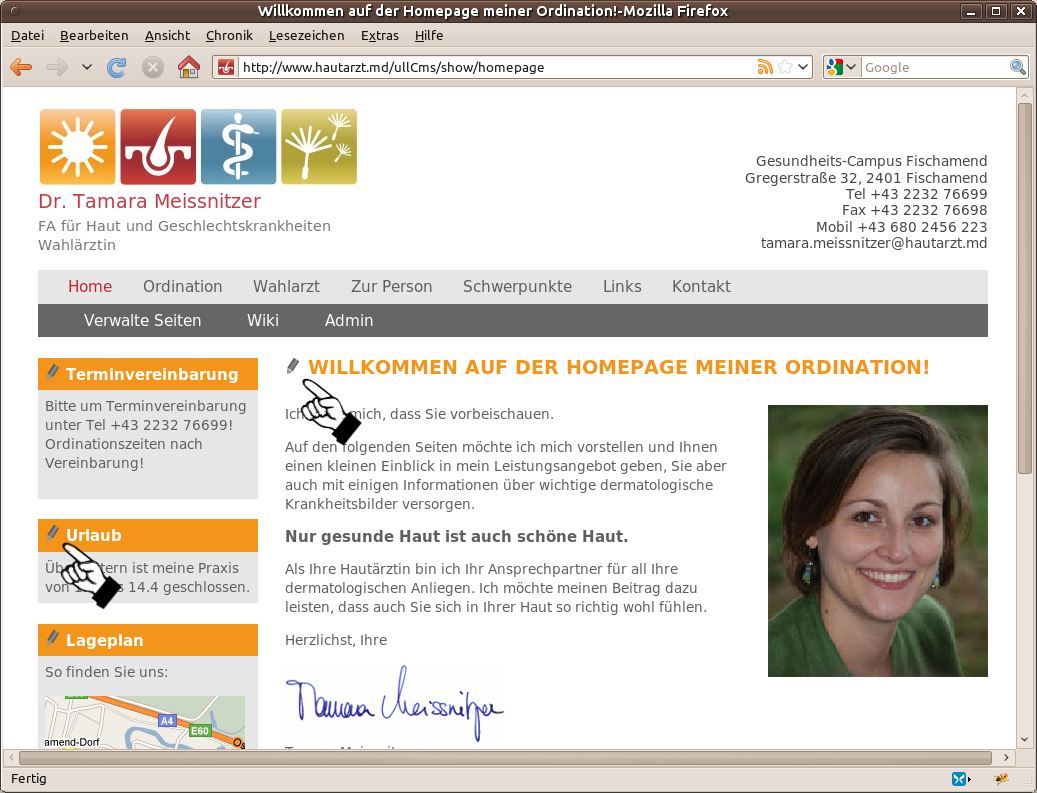
\includegraphics[width=0.9\textwidth]{direct_edit}
\caption{Icons zur direkten Bearbeitung}
\label{fig:direct_edit}
\end{figure}

Wenn Sie angemeldet sind und die nötigen Berechtigungen besitzen erscheint praktischerweise vor jedem bearbeitbaren Inhalt ein Stiftsymbol (Icon) (Siehe Abbildung \vref{fig:direct_edit}). Durch Klick auf das Icon können Sie den entsprechenden Text sofort bearbeiten.
Näheres zur Bearbeitung selbst erfahren Sie im Kapitel \vref{sec:edit}.




\section{Inhaltsverwaltung}

Klicken Sie in der Admin-Menüleiste auf den Menüpunkt "`Inhalte verwalten"'. 

Als Modul der ullright Plattform ist die `Startseite` wie üblich aufgebaut (Abbildung \vref{fig:index}):

\begin{figure}[htp]
\centering
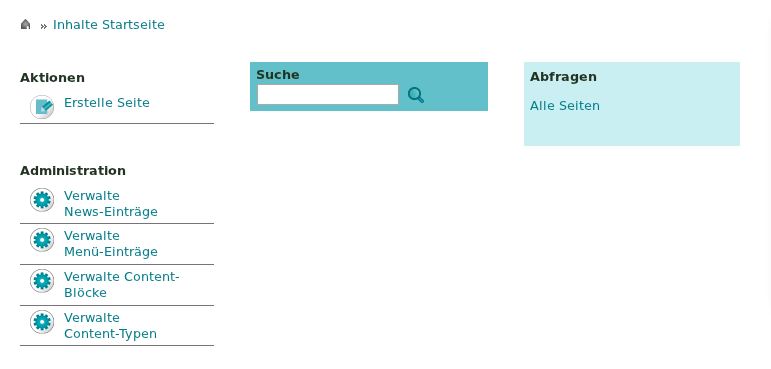
\includegraphics[width=0.9\textwidth]{index}
\caption{Startseite der Inhaltsverwaltung}
\label{fig:index}
\end{figure}

\subsection{Neue Seite erstellen}

Klicken Sie auf der auf "`Erstelle Seite"' um eine neue CMS-Seite zu erstellen. Alles weitere erfahren Sie im Kapitel \vref{sec:edit}.

\subsection{Administration - Verwalte News-Einträge}

Erlaubt Ihnen die Verwaltung von Newseinträgen auf Ihrer Homepage. Nur sichtbar, wenn das ullNews Modul aktiviert ist.

\subsection{Administration - Verwalte Menü-Einträge}

Erstellen oder Bearbeiten vom Menüeinträgen. Betroffen sind nur Menüeinträge die keine Seite sind, also keinen Inhalt haben.
Beispiele: "`Hauptmenü"', "`Fußzeile"', etc.

\subsection{Administration - Verwalte Content-Blöcke}

Siehe Kapitel \vref{sec:contentblock}.

\subsection{Suche}

Wenn Ihre Webseite aus vielen Seiten besteht kann die Suchfunktion (Abbildung \vref{fig:search}) hilfreich sein .

Geben Sie eine Suchbegriff oder auch nur einen Teil davon in das Suchfeld ein und drücken Sie $\Enter$ oder klicken Sie das Lupen-Symbol an.
Die Liste beschränkt sich nun auf die Seiten, die den Suchbegriff im Betreff enthalten. Der Suchbegriff erscheint zusätzlich als "`Filter"'. Durch Klick auf das Papierkorb-Symbol entfernen Sie das Filterkriterium.

\subsection{Abfragen}

Klicken Sie hier um eine Liste aller Seiten anzuzeigen. Siehe Kapitel \vref{sec:edit}.

\section{Liste aller Seiten}

Sie sehen eine Liste aller CMS-Seiten (Abbildung \vref{fig:list}):

\begin{figure}[htp]
\centering

\includegraphics[width=0.9\textwidth]{list}
\caption{Liste aller CMS-Seiten}
\label{fig:list}
\end{figure}


\subsection{Spalten}

Folgende Spalten werden üblicherweise in der Liste angezeigt:

\begin{itemize}
\item Titel der Seite
\item Übergeordneter Menüeintrag - Also wo die Seite in der Struktur der Webseite plaziert ist. Beispiele: "`Hauptmenü"', "`Fußzeile"' oder als Untermenüpunkt wie z.B. die Seite "`Anfängerkurse"' als Unterpunkt von "`Kurse"'.
\item Ist aktiv - Der Status der Seite. Inaktive Seiten werden den Besuchern nicht angezeigt.
\item Aktualisiert von - Wer die Seite zuletzt bearbeitet hat
\item Aktualisiert am - Wann die Seite zuletzt bearbeitet wurde
\end{itemize}


\subsection{Sortieren}

Klicken Sie auf eine Spaltenüberschrift wie zum Beispiel "`Aktualisiert am"' um die Liste nach diesem Feld zu sortieren. Klicken Sie nochmal auf die gleiche Spaltenüberschrift um die Sortierung umzukehren.


\subsection{Blättern}

Bei einer großen Anzahl an Seiten werden nicht alle Einträge auf einer Seite angezeigt. Benutzen Sie in diesem Fall die "`Blättern"' Funktion um weitere Seiten aufzurufen (Abbildung \vref{fig:paging}).

\begin{figure}[htp]
\centering
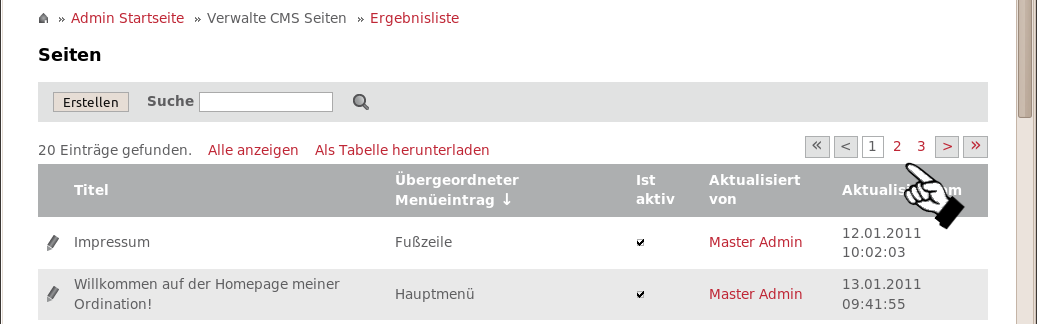
\includegraphics[width=0.9\textwidth]{paging}
\caption{Blättern}
\label{fig:paging}
\end{figure}


\subsection{Suche}

Wenn Ihre Webseite aus vielen Seiten besteht kann die Suchfunktion (Abbildung \vref{fig:search}) hilfreich sein .

Geben Sie eine Suchbegriff oder auch nur einen Teil davon in das Suchfeld ein und drücken Sie $\Enter$ oder klicken Sie das Lupen-Symbol an.
Die Liste beschränkt sich nun auf die Seiten, die den Suchbegriff im Betreff enthalten. Der Suchbegriff erscheint zusätzlich als "`Filter"'. Durch Klick auf das Papierkorb-Symbol entfernen Sie das Filterkriterium.

\begin{figure}[htp]
\centering
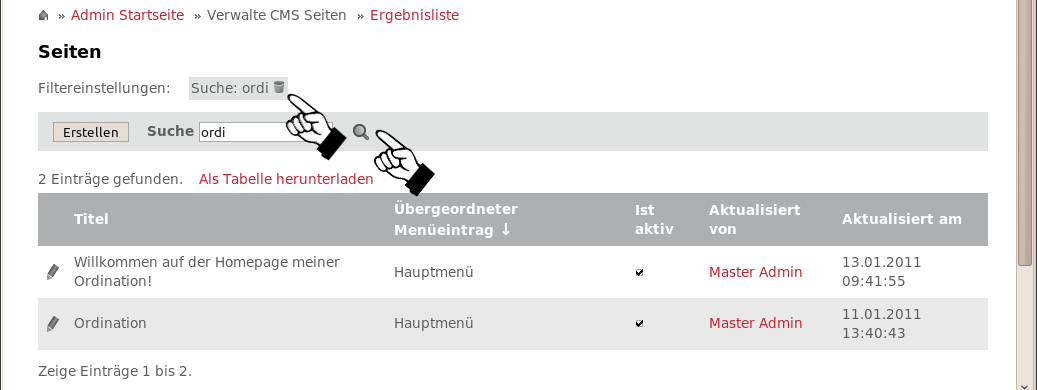
\includegraphics[width=0.9\textwidth]{search}
\caption{Suche}
\label{fig:search}
\end{figure}



\subsection{Neue Seite erstellen}

Klicken Sie auf der auf "`Erstellen"' um eine neue CMS-Seite zu erstellen. Alles weitere erfahren Sie im Kapitel \vref{sec:edit}.


\section{Seiten bearbeiten}
\label{sec:edit}

Eine der Stärken von ullCms ist, dass es komplett an die Bedürfnisse des Kunden angepasst werden kann.
Deshalb werden sich die Datenfelder Ihrer Installation wahrscheinlich von dieser Dokumentation unterscheiden. Im folgenden werden häufig eingesetze Felder behandelt.

\begin{figure}[htp]
\centering
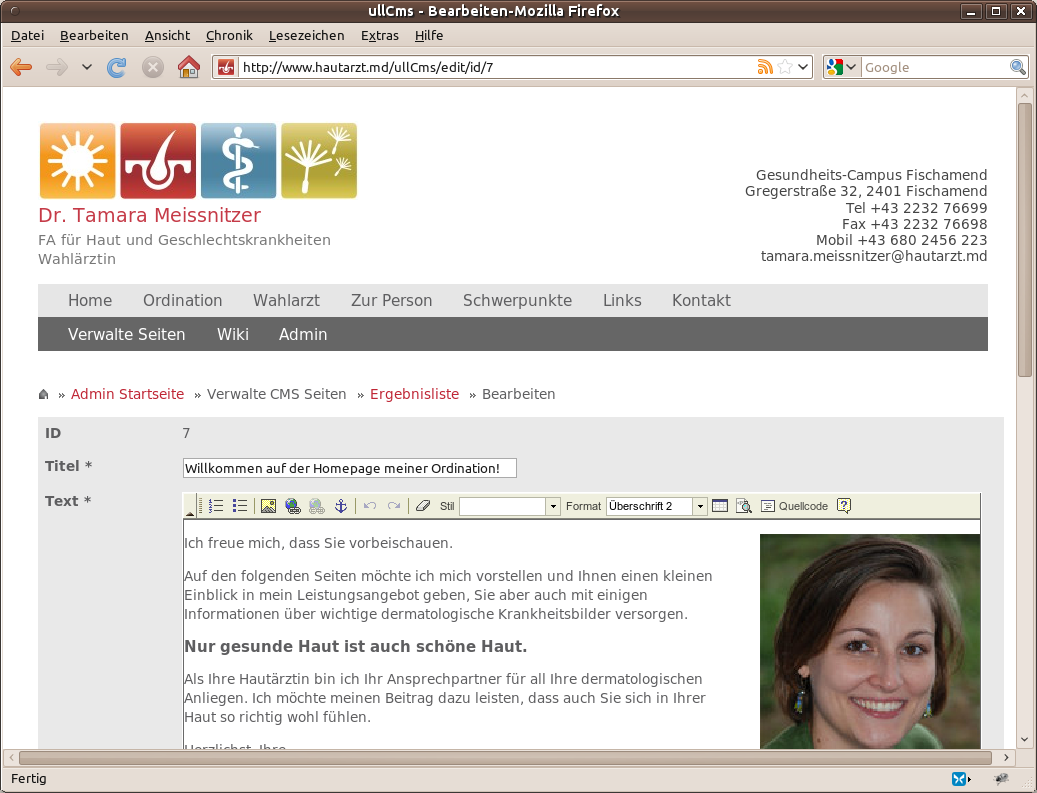
\includegraphics[width=0.9\textwidth]{edit1}
\caption{Bearbeiten Teil 1}
\label{fig:edit1}
\end{figure}

\begin{figure}[htp]
\centering
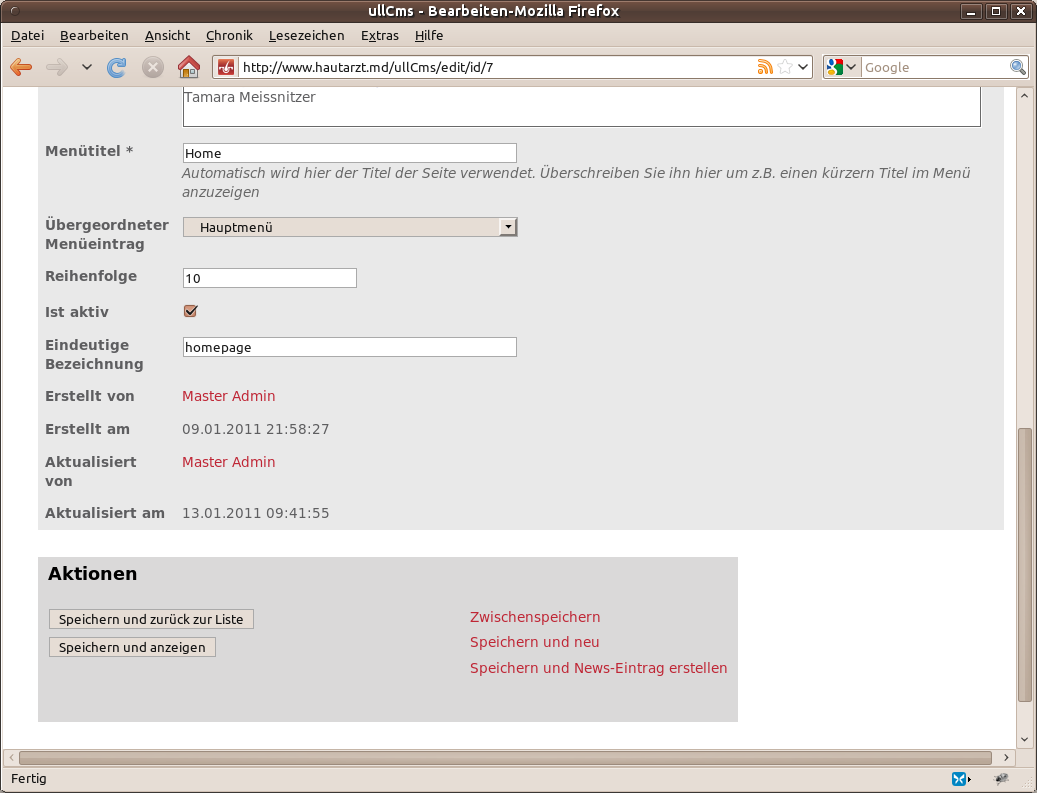
\includegraphics[width=0.9\textwidth]{edit2}
\caption{Bearbeiten Teil 2}
\label{fig:edit2}
\end{figure}

\subsection{Titel}

Der Titel Ihrer Seite wie er auf der Seite selbst als Überschrift angezeigt werden soll.

\subsection{Menütitel}

Der Titel des Seite für die Anzeige im Menü. Standardmäßig wird hier der Titel übernommen. Es kann aber sinnvoll sein einen kürzeren Text für die Menüs zu verwenden.

\subsection{Text}

ullCms bietet einen komfortablen
Editor (FCK- bzw CK-Editor), der ähnlich wie OpenOffice Writer oder MS Word funktioniert.
Auch das Einfügen von Bildern oder Anhängen ist einfach möglich. 

Alles rund um die Bedienung des Editors erfahren Sie im Kapitel \vref{sec:editor}.

\subsection{Bild}

Je nach Ihrer Konfiguration können ein oder mehrere separate Felder für Bilder vorhanden sein.

Beispiele:

\begin{itemize}
\item Bild, dass an einer bestimmten Stelle der Seite angezeigt wird
\item Vorschaubilder z.B. bei Produkten
\end{itemize}

Sie brauchen sich nicht um die Größe des Bildes zu kümmern. Die Bilder werden automatisch passend skaliert.
Auch der Speicherort wird automatisch gewählt.

\subsection{Galerie / Multi-Upload}
\label{sec:gallery}

Besonders benutzerfreundlich ist die Funktion zum Hochladen mehrerer Bilder z.B: für eine Galerie.

Highlights:
\begin{itemize}
\item Mehrere Bilde auf einmal auswählen und hochladen
\item Unter Firefox sogar mittels Drag'n'Drop: Einfach mehrere Bilder im Explorer markieren und in den Webbrowser ziehen und dort fallen lassen
\item Die Bilder werden automatisch skaliert
\item Kleine Vorschaubilder werden automatisch erstellt
\item Die Bilder können mit der Maus in die richtige Reihenfolge gezogen werden.
\item Auch andere Dateien wie z.B. PDF, Word, Excel, OpenOffice usw. werden unterstützt und sogar ein Vorschaubild wird automatisch generiert.
\end{itemize}


\begin{figure}[htp]
\centering
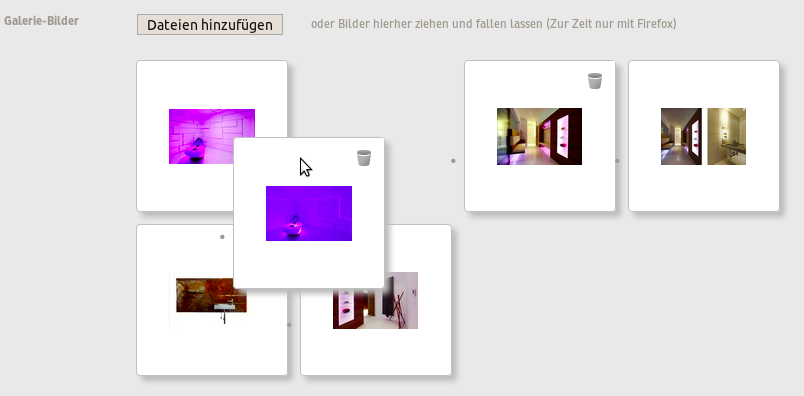
\includegraphics[width=0.9\textwidth]{gallery}
\caption{Galerie / Multi-Upload}
\label{fig:gallery}
\end{figure}






\subsection{Übergeordneter Menüeintrag}

Wählen Sie hier an welchem Punkt der Struktur Ihrer Webseite die aktuelle Seite plaziert wird. Beispiele: "`Hauptmenü"', "`Fußzeile"' oder als Untermenüpunkt wie z.B. die Seite "`Anfängerkurse"' als Unterpunkt von "`Kurse"'.

\subsection{Reihenfolge}

Normalerweise werden die einzelnen Einträge in einem Menü wie z.B. dem Hauptmenü alphabetisch sortiert. In dieses Feld können sie ganze Zahlen eingeben um die Sortierung zu beeinflussen. Tipp: verwenden sie ganze 10er oder 100er Zahlen um später Einträge einfügen zu können. 

\subsection{Tags / Schlagworte}
\label{sec:tagging}

Sie können Ihren Seiten mittels Tags kategorisieren. Diese sind dann sowohl in der Suche als auch für erweiterte Features wie z.B. der Vorschlags-Funktion (siehe Kapitel \vref{sec:recommendation}) auswertbar.

\begin{figure}[htp]
\centering
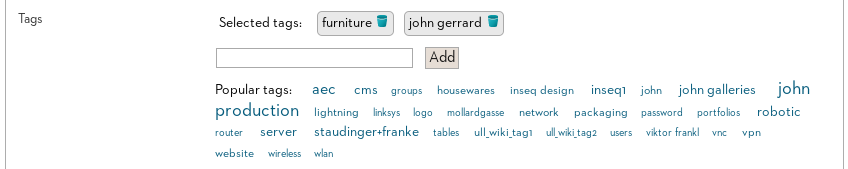
\includegraphics[width=0.9\textwidth]{tagging}
\caption{Tagging}
\label{fig:tagging}
\end{figure}

Geben Sie einen neues Schlagwort ein und klicken Sie auf "`Hinzufügen, oder klicken Sie auf ein bereits vorhandenes Schlagwort in der "'Tag-Cloud"`.

Ein Klick auf das Papierkorb-Symbol entfernt ein gewähltes Schlagwort.

\subsection{Ist aktiv}

Der Status der Seite. Setzen Sie den Status auf "`Inaktiv"' um eine Seite den Besuchern nicht mehr anzuzeigen.




\subsection{Weitere Felder anzeigen}

Klicken Sie auf "`Weitere Felder anzeigen"' um selten benötigte Felder zu bearbeiten.

\subsubsection{Eindeutige Bezeichnung}

Der Name der Seite wie er in der Adresszeile (URL) angezeigt wird. Beispiel: "'anfaenger-kurse"`.

\subsubsection{Erstellt von/am}

Wer und wann die Seite erstellt hat.

\subsubsection{Zuletzt bearbeitet von/am}

Wer und wann die Seite zuletzt bearbeitet hat.



\subsection{Aktionen}

Für das Bearbeiten oder Erstellen mehrerer Seiten bietet ullCms einige praktische Aktionen:

\begin{itemize}
\item Speichern und zurück zur Liste - Sie gelangen wieder zur Liste der Seiten
\item Speichern und anzeigen - Die eben bearbeitete Seite aus der Sicht der Besucher ansehen
\item Zwischenspeichern - Auf der Bearbeitunsseite bleiben
\item Speichern und neu - Unmittelbar mit der Eingabe der Inhalte einer neuen Seite beginnen
\item Speichern und News-Eintrag erstellen - Wenn Sie das ullNews Modul verwenden können Sie hier direkt einen neuen News-Eintrag erstellen der zur eben bearbeiteten CMS-Seite verlinkt ist
\end{itemize}



\section{Text bearbeiten mit dem "`WYSIWYG"' Editor}
\label{sec:editor}

"`WYSIWYG"' steht für "`What you see is what you get"',  also dass man schon bei der Eingabe sieht wie der Text letztendlich aussehen wird.

Die angezeigten Formatierungs-Möglichkeiten können sich je nach Konfiguration und Editor-Version von Ihrer Installation unterscheiden.

\begin{figure}[htp]
\centering
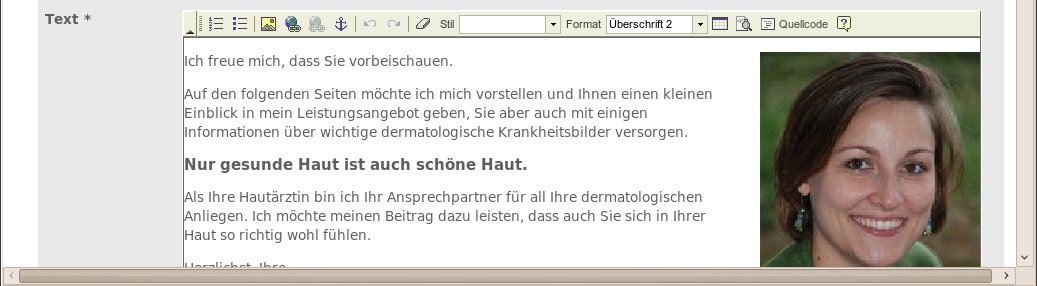
\includegraphics[width=0.9\textwidth]{editor}
\caption{WYSIWYG-Editor}
\label{fig:editor}
\end{figure}

\subsection{Text schreiben}

Geben Sie wie von anderen Texteditoren gewohnt den Text ein.

Tipp: $\Enter$ erzeugt einen neuen Paragrafen, also einen Textblock mit einer Leerzeile dahinter. Einen einfachen Zeilenumbruch erreichen Sie mit $\Shift + \Enter$.

\subsection{Text formatieren}

Markieren Sie den gewünschten Text und wählen Sie aus der Editor-Menüleiste die gewünschte Auszeichnung.

Bitte beachten Sie, dass die von uns ausgewählten
Formatierungsmöglichkeiten nach semantischen Gesichtspunkten ausgewählt
wurden. Sie finden also nur „logische“ Auszeichnungen wie zum Beispiel
„wichtig“ oder „Überschrift“, und keine rein optischen
Formatierungsmöglichkeiten wie Farben oder Schriftgrößen. Somit werden
saubere und zukunftssichere Texte gewährleistet. (Stichwort "`semantic
Web"')

Die wichtigsten Formatierungen (von links nach rechts):

\begin{itemize}
\item Nummerierte Liste
\item Liste mit Aufzählungszeichen
\item Stile: "`Important"' -- also "`Wichtig"' wird fett angezeigt
\item Format: "`Überschrift"'
\end{itemize}


\subsection{Bild einfügen}

\begin{itemize}
\item Setzten Sie den Cursor an die gewünschte Stelle im Text
\item Klicken Sie auf das Bildsymbol 
\includegraphics[height=5mm]{image_icon}
\item Wählen Sie "`Server durchsuchen"'
\item Wählen oder erstellen Sie gegebenenfalls einen neuen Ordner um eine ordentliche Struktur Ihrer Daten zu gewährleisten
\item Wenn Sie ein neues Bild hochladen möchten klicken Sie auf "`Durchsuchen"' und wählen Sie eine Bilddatei von Ihrem Computer aus.
\item Vergessen Sie nicht danach auf "`Upload"' zu klicken
\item Wählen Sie nun ein Bild aus der Liste durch anklicken.
\item Klicken Sie auf "`OK"'
\end{itemize}

\subsection{Bildeigenschaften ändern}

Klicken Sie mit der rechten Maustaste auf das Bild und wählen Sie "`Bildeigenschaften"'.

Im folgenden werden die wichtigsten Eigenschaften erklärt:

\subsubsection{Reiter "`Bild-Info"'}

\begin{itemize}
\item Breite / Höhe - Wählen Sie die gewünschte Größe des Bildes in Pixel. Bitte beachten Sie, dass Bilder bereits vor dem Hochladen mit einem Grafikprogramm auf die endgültige Größe skaliert werden sollten
\item Ausrichtung - Wählen Sie "`Links"' oder "`Rechts"' wenn der Text das Bild umfließen soll.
\end{itemize}

\subsubsection{Reiter "`Erweitert"'}

Wenn Sie das Bild vom Text umfließen lassen ist häufig auf gewissen Seiten des Bildes ein Abstand erwünscht.
Dieser Abstand kann im Feld "`Style"' angegeben werden. Beispiel für einen Abstand links und unten: "`margin-left: 1.5em; margin-bottom: 1.5em;"'


\subsection{Link erstellen}

Normale Webadressen und E-Mailadressen werden in der normalen Ansicht für die Besucher der Webseite automatisch verlinkt.

Beispiele:

\begin{itemize}
\item www.ullright.org
\item http://ull.at
\item office@ull.at
\end{itemize}

Möchten Sie hingegen gewisse Wörter im Text verlinken markieren Sie die Wörter und klicken Sie auf das Linksymbol 
\includegraphics[height=5mm]{link_icon} (blau-grüne Erdkugel).

\subsubsection{Link zu einer Internetadresse (URL)}
Geben Sie bei "`URL"' die gewünschte Adresse ein. Beispiel: \url{http://www.ullright.org}

Bei Links zu Internetseiten empfiehlt sich die Seite in einem neuen Browserfenster zu öffnen. Wählen Sie hierzu im Reiter "`Zielseite"' "`Neues Fenster (\_blank)"'.

Zusätzlich empfehlen wir einen solchen Link durch das Symbol für "`Externe Seite"' zu kennzeichen. Schreiben Sie dazu im Reiter "`Erweitert"' die Anweisung "`link\_external"' in das Feld "`Stylesheet Klasse"'.

\subsubsection{Link zu einer anderen CMS-Seite}

Öffnen Sie die Zielseite in einem neuen Browsertab oder -fenster und kopieren Sie die URL aus der Adressleiste.

Beispiel: \url{http://www.ull.at/ullCms/show/kontakt}

Geben Sie nun bei "`URL"' die gekürzte Adresse startend mit den Schrägstrich nach dem Domänennamen ein.

Beispiel: \url{/ullCms/show/kontakt}

\subsubsection{E-Mail Link}

Wählen Sie bei "`Link-Typ"' E-Mail und geben Sie die gewünschte E-Mailadresse ein.



\subsection{Datei hochladen}
\label{sec:upload_file}

Das Hochladen einer Datei funktioniert wie eine Mischung aus Link- und Bildeinfügen.

\begin{itemize}
\item Markieren Sie die Wörter die mit der Datei verlinkt werden sollen
\item Klicken Sie auf das Linksymbol 
\includegraphics[height=5mm]{link_icon}
\item Wählen Sie „Server durchsuchen“
\item Wählen oder erstellen Sie gegebenenfalls einen neuen Ordner um eine ordentliche Struktur Ihrer Daten zu gewährleisten
\item Wenn Sie eine neue Datei hochladen möchten klicken Sie auf "`Durchsuchen"' und wählen Sie eine Datei von Ihrem Computer aus
\item Vergessen Sie nicht danach auf "`Upload"' zu klicken
\item Wählen Sie nun die Datei aus der Liste durch anklicken
\item Klicken Sie auf "`OK"'
\end{itemize}


\subsection{Tip für PDF-Dateien}

Auf vielen PCs wird bei einem Klick auf den Link zu einer PDF-Datei das PDF direkt im Browserfenster geöffnet. Besuchern passiert es dann häufig, dass sie nach dem Lesen das Fenster oder Tab einfach schließen, und somit auch Ihre Website verlassen.

Um diesem unerwünschten Verhalten vorzubeugen empfiehlt sich ein PDF in einem Pop-up Fenster zu öffnen:

\begin{itemize}
\item Verlinken Sie eine PDF-Datei wie im Kapitel \vref{sec:upload_file} beschrieben
\item Klicken Sie mit der rechten Maustaste auf den Link zur PDF-Datei und wählen Sie "`Link editieren"'
\item Im Reiter "`Zielseite"' wählen Sie nun "`Pop-up Fenster"'
\item Haken Sie die Felder "`Vergrößerbar"', "`Adress-Leiste"', "`Menüleiste"' und "`Rollbalken"' an.
\item Schließen Sie den Vorgang mit "`OK"' ab.
\end{itemize}


\section{Erweiterte Funktionen}

\subsection{Content-Blöcke}
\label{sec:contentblock}

Erstellen und Bearbeiten von Content-Blöcken. Content-Blöcke sind direkt bearbeitebare Inhaltsbereiche die keine Seite im eigentlichen Sinne sind.

Beispiele:

\begin{itemize}
\item Auf mehreren Seiten wiederkehrende Elemente wie z.B. Sidebar-Blöcke
\item Elemente einer komplexen Seite die aus mehreren Bereichen aufgebaut
\item Strukturierte Elemente die mehrfach vorkommen wie z.B. Team-Mitglieder
\end{itemize}

\begin{figure}[htp]
\centering

\includegraphics[width=0.9\textwidth]{content_block_show}
\caption{Content Blöcke für strukturierte Inhalte (Partner)}
\label{fig:content_block_show}
\end{figure}

Siehe auch Abbildung \vref{fig:direct_edit}). Dort sind Content-Blöcke auf der linken Seite ersichtlich ("`Terminvereinbarung"', "`Urlaub"', ...).

Die Verwaltung ist ganz einfach, da jeder Content-Block ähnlich wie eine normale CMS-Seite behandelt wird.
Allerding lässt sich die Bearbeitungsseite (welche Felder, welche Editor-Optionen, ...) eigens konfigurieren.


\subsection{Menüstruktur}

ullCms verwendet eine sehr flexible Menüstruktur. 

Beispiel für eine typische Struktur:

\subsubsection{Hauptmenü}

Das Hauptmenü mit Menüpunkten wie z.B. Home, Über uns, Produkte, Kontakt, usw


\subsubsection{Fußzeile}

Einträge am unteren Ende der Seite wie z.B. Impressum, AGB, ...

\subsubsection{Unsichtbar - scheint in keinem Menü auf}

Hier können Sie Seiten plazieren die in keinem der oben genannten Menüs aufscheinen soll. Dies kann verwendet werden um z.B. eine Spezialseite für eine E-Mail Aussendung zu erstellen.

\subsubsection{Papierkorb - Für nicht mehr aktuelles}

Verschieben Sie veraltete oder nicht mehr benötigte Seiten hierher um Ihre Menüstruktur sauber zu halten


\subsection{Vorschlagsfunktion}
\label{sec:recommendation}

Die Auswahl von Tags (Schlagworten - siehe auch Kapitel \vref{sec:tagging}) für einzelne Seiten kann z.B. im Fall von Produktseiten für eine Vorschlags-Funktion verwendet werden. Auf einer Seite werden dabei verwandte Seiten vorgeschlagen. Dies wird über die Vergabe von gleichen Tags gesteuert

\begin{figure}[htp]
\centering
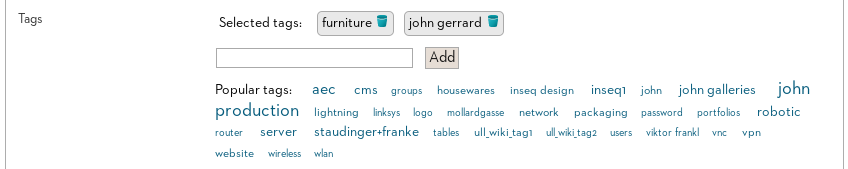
\includegraphics[width=0.9\textwidth]{tagging}
\caption{Gewählte Schlagworte für die Vorschlagsfunktion)}
\label{fig:tagging2}
\end{figure}

\begin{figure}[htp]
\centering
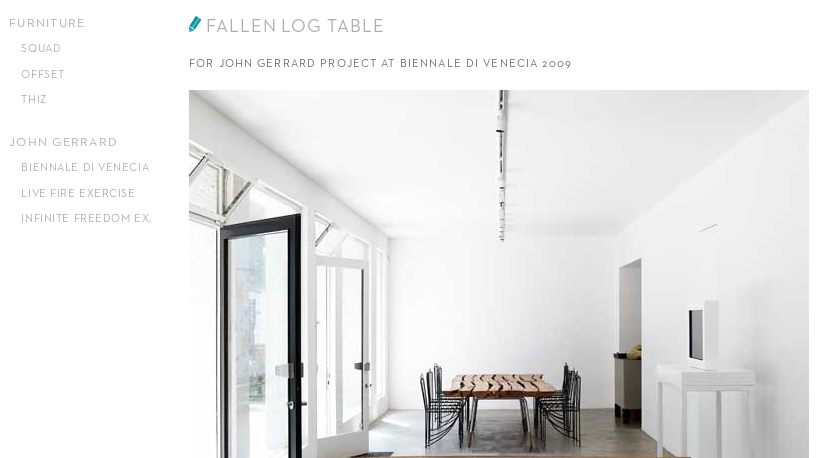
\includegraphics[width=0.9\textwidth]{recommendation}
\caption{Vorschläge für verwandte Seiten mittels der Vergabe gleicher Schlagworte (auf der linken Seite)}
\label{fig:recommendation}
\end{figure}



\section{Quellenangaben}

Danke an folgende ull.at Kunden, die Screenshots ihrer Webseiten zur Verfügung stellten:

\begin{itemize}
\item Andreas Etzelstorfer - \href{http://www.backraum.at}{www.backraum.at}
\item Dr. Tamara Meissnitzer - \href{http://www.hautarzt.md}{www.hautarzt.md}
\item INSEQ DESIGN - \href{http://www.inseq.com}{www.inseq.com}
\item ullright Demoseite - \href{http://demo.ullright.org}{demo.ullright.org}
\end{itemize}




\end{document}